% <#>--------------------------------------------------<#>
\section{Vorwort}%
\label{sec:vorwort}

Flucky ist ein Webserver, geschrieben in der Programmiersprache
\href{https://golang.org/}{Go} (Golang). Dabei ist zu differenzieren zwischen
dem Flucky-Server und der Flucky-CLI. Die Server Version nimmt Daten von Clients
mittels REST entgegen und speichert diese in einer Datenbank ab. Die Flucky-CLI
ist ein Client der die REST-API des Flucky-Servers nutzt um Daten zu
übermitteln.

Die API des Flucky-Servers ist dokumentiert und kann auch durch alternative
CLI-Programme die REST beherrschen angesteuert werden.

Der Quellcode der beiden Projekte stehen unter Apache 2.0
Lizenz \footcite{apache-licence} und sind auf
\href{https://git.cryptic.systems}{git.cryptic.systems} gehostet.

% <#>--------------------------------------------------<#>
\section{Einleitung}%
\label{sec:einleitung}

\begin{wrapfigure}{R}{0.4\textwidth}
  
\includegraphics[width=0.4\textwidth]{img/flucky.png}
  \caption{Flucky-Maskottchen}
\end{wrapfigure}

Der Flucky-Webserver ist in der Programmiersprache Go (Golang) geschrieben und
nutzt \Gls{gls:rest} als Kommunikation zwischen den Clients.

Dabei ergeben sich mehrere \Gls{gls:rest}-Endknoten, an die der Client mittels
unterschiedlichen HTTP-Anfragemethoden seine Daten schicken kann.

Als Datenstruktur wird \Gls{gls:json} genutzt. Eine Beschreibung der
JSON-Strukturen befindet sich in der
\href{https://git.cryptic.systems/fh-trier/go-flucky-server/wiki}{Dokumentation}
des Flucky-Servers.

Da der Server für Cloud-Architekturen entwickelt wurde, befindet sich in Kapitel
Installation von Docker nicht nur eine Dokumentation der Installation des
Servers, sondern auch eine wie der Server skaliert werden kann.

% <#>------------------------------------------------<#>
\section{REST-Endknoten - HTTP-Anfragemethoden}%
\label{sec:rest}

\acrfull{acr:rest} bezeichnet ein Programmierparadigma für verteilte Systeme,
insbesondere Webservices. Daher ist eine Implementierung nach
\acrshort{acr:rest} sehr Sinnvoll, zu mal es sich bei solchen Daten oft um
zustandslosen Daten\footcite{zustandslosigkeit} handelt.

Es bietet die Möglichkeit mehrere Webservices auszuführen um die Last zu
skalieren, sofern die einzelnen Geräte mit ihren Sensoren eine so hohe Datenflut
erzeugen, dass ein einzelner Service unter den Anfragen zum erliegen kommen
würde. Bei solch einem Szenario würde man von einem \Gls{gls:ddos}-Angriff
sprechen.

Dabei bietet der Flucky-Webserver mehrere \acrshort{acr:rest}-Endknoten an, die
auf unterschiedliche \Gls{gls:http-anfragemethoden} reagieren um nach dem
\Gls{gls:crud}-Ansatz zu arbeiten.

Nachfolgend sind alle \acrshort{acr:rest} -Endknoten mit Anfragemethode
gelistet, dabei werden folgende Anfragemethoden vom Flucky-Server verwendet und
stehen Clients zur Verfügung.

\begin{description}[itemsep=0pt]
  \item[POST] Übergibt eine neue Ressource. Gleicht dem INSERT von RDBM-Systemen oder dem C (Create) des \acrshort{acr:crud}-Ansatzes.
  \item[GET] Gibt eine Ressource zurück. Ähnelt dem SELECT von RDBM-Systemen oder dem R (Read) aus dem \acrshort{acr:crud}-Ansatz.
  \item[PUT] Aktualisiert eine existierende Ressource. Ähnelt dem UPDATE von RDBM-Systemen und steht gleichnahmig für das U im \acrshort{acr:crud}-Ansatz.
  \item[DELETE] Löscht eine Ressource. Gleicht dem DELETE von RDBM-Systemen und steht gleichnahmig für das D im \acrshort{acr:crud}-Ansatz.
\end{description}

\begin{landscape}
  \begin{table}[H]
    \begin{longtable}{lllllll}
      \textbf{Typ}                    & \textbf{REST-Knoten}                    & \textbf{POST} & \textbf{GET} & \textbf{PUT} & \textbf{DELETE} & \textbf{Beschreibung}   \\ \toprule
      \multirow{5}{*}{Camera Equals}  & /camera\_equals                         & X & X &   & X & Delete löscht ALLE Einträge                                             \\
                                      & /camera\_equals/$\{$datum$\}$           &   & X &   & X & Datum im Format YYYY-MM-DD                                              \\
                                      & /camera\_equals/$\{$von$\}$/$\{$bis$\}$ &   & X &   & X & Datum im Format YYYY-MM-DD                                              \\
                                      & /camera\_equals/$\{$id$\}$              & X &   & X & X & Die ID ist eine UUID                                                    \\
                                      & /camera\_equals/$\{$sensor\_id$\}$      &   & X &   & X & Die ID ist eine UUID                                                    \\ \midrule
      \multirow{5}{*}{Camera Sizes}   & /camera\_sizes                          & X & X &   & X & Delete löscht ALLE Einträge                                             \\
                                      & /camera\_sizes/$\{$datum$\}$            &   & X &   & X & Datum im Format YYYY-MM-DD                                              \\
                                      & /camera\_sizes/$\{$von$\}$/$\{$bis$\}$  &   & X &   & X & Datum im Format YYYY-MM-DD                                              \\
                                      & /camera\_sizes/$\{$id$\}$               & X &   & X & X & Die ID ist eine UUID                                                    \\
                                      & /camera\_sizes/$\{$sensor\_id$\}$       &   & X &   & X & Die ID ist eine UUID                                                    \\ \midrule
      \multirow{3}{*}{Devices}        & /devices                                & X & X &   & X & Delete löscht ALLE Einträge                                             \\
                                      & /camera\_sizes/$\{$id$\}$               & X &   & X & X & Die ID ist eine UUID                                                    \\
                                      & /camera\_sizes/$\{$sensor\_id$\}$       &   & X &   & X & Die ID ist eine UUID                                                    \\ \midrule
      \multirow{5}{*}{Failnoises}     & /failnoises                             & X & X &   & X & Delete löscht ALLE Einträge                                             \\
                                      & /failnoises/$\{$datum$\}$               &   & X &   & X & Datum im Format YYYY-MM-DD                                              \\
                                      & /failnoises/$\{$von$\}$/$\{$bis$\}$     &   & X &   & X & Datum im Format YYYY-MM-DD                                              \\
                                      & /failnoises/$\{$id$\}$                  & X &   & X & X & Die ID ist eine UUID                                                    \\
                                      & /failnoises/$\{$sensor\_id$\}$          &   & X &   & X & Die ID ist eine UUID                                                    \\ \midrule
    \end{longtable}
  \end{table}

  \newpage

  \begin{table}[H]
    \begin{longtable}{lllllll}
      \textbf{Typ}                    & \textbf{REST-Knoten}                    & \textbf{POST} & \textbf{GET} & \textbf{PUT} & \textbf{DELETE} & \textbf{Beschreibung}   \\ \toprule
      \multirow{5}{*}{Humidities}     & /humidities                             & X & X &   & X & Delete löscht ALLE Einträge                                             \\
                                      & /humidities/$\{$datum$\}$               &   & X &   & X & Datum im Format YYYY-MM-DD                                              \\
                                      & /humidities/$\{$von$\}$/$\{$bis$\}$     &   & X &   & X & Datum im Format YYYY-MM-DD                                              \\
                                      & /humidities/$\{$id$\}$                  & X &   & X & X & Die ID ist eine UUID                                                    \\
                                      & /humidities/$\{$sensor\_id$\}$          &   & X &   & X & Die ID ist eine UUID                                                    \\ \midrule
      \multirow{5}{*}{Knocks}         & /knocks                                 & X & X &   & X & Delete löscht ALLE Einträge                                             \\
                                      & /knocks/$\{$datum$\}$                   &   & X &   & X & Datum im Format YYYY-MM-DD                                              \\
                                      & /knocks/$\{$von$\}$/$\{$bis$\}$         &   & X &   & X & Datum im Format YYYY-MM-DD                                              \\
                                      & /knocks/$\{$id$\}$                      & X &   & X & X & Die ID ist eine UUID                                                    \\
                                      & /knocks/$\{$sensor\_id$\}$              &   & X &   & X & Die ID ist eine UUID                                                    \\ \midrule
      \multirow{5}{*}{Particulates10} & /particulates10                         & X & X &   & X & Delete löscht ALLE Einträge                                             \\
                                      & /particulates10/$\{$datum$\}$           &   & X &   & X & Datum im Format YYYY-MM-DD                                              \\
                                      & /particulates10/$\{$von$\}$/$\{$bis$\}$ &   & X &   & X & Datum im Format YYYY-MM-DD                                              \\
                                      & /particulates10/$\{$id$\}$              & X &   & X & X & Die ID ist eine UUID                                                    \\
                                      & /particulates10/$\{$sensor\_id$\}$      &   & X &   & X & Die ID ist eine UUID                                                    \\ \midrule
      \multirow{5}{*}{Particulates25} & /particulates25                         & X & X &   & X & Delete löscht ALLE Einträge                                             \\
                                      & /particulates25/$\{$datum$\}$           &   & X &   & X & Datum im Format YYYY-MM-DD                                              \\
                                      & /particulates25/$\{$von$\}$/$\{$bis$\}$ &   & X &   & X & Datum im Format YYYY-MM-DD                                              \\
                                      & /particulates25/$\{$id$\}$              & X &   & X & X & Die ID ist eine UUID                                                    \\
                                      & /particulates25/$\{$sensor\_id$\}$      &   & X &   & X & Die ID ist eine UUID                                                    \\ \midrule
    \end{longtable}
  \end{table}

  \newpage

  \begin{table}[H]
    \begin{longtable}{lllllll}
      \textbf{Typ}                    & \textbf{REST-Knoten}                  & \textbf{POST} & \textbf{GET} & \textbf{PUT} & \textbf{DELETE} & \textbf{Beschreibung}     \\ \toprule
      \multirow{5}{*}{Temperatures}   & /temperatures                         & X & X &   & X & Delete löscht ALLE Einträge                                               \\
                                      & /temperatures/$\{$datum$\}$           &   & X &   & X & Datum im Format YYYY-MM-DD                                                \\
                                      & /temperatures/$\{$von$\}$/$\{$bis$\}$ &   & X &   & X & Datum im Format YYYY-MM-DD                                                \\
                                      & /temperatures/$\{$id$\}$              & X &   & X & X & Die ID ist eine UUID                                                      \\
                                      & /temperatures/$\{$sensor\_id$\}$      &   & X &   & X & Die ID ist eine UUID                                                      \\ \midrule
      \multirow{5}{*}{Throughputs}    & /throughputs                          & X & X &   & X & Delete löscht ALLE Einträge                                               \\
                                      & /throughputs/$\{$datum$\}$            &   & X &   & X & Datum im Format YYYY-MM-DD                                                \\
                                      & /throughputs/$\{$von$\}$/$\{$bis$\}$  &   & X &   & X & Datum im Format YYYY-MM-DD                                                \\
                                      & /throughputs/$\{$id$\}$               & X &   & X & X & Die ID ist eine UUID                                                      \\
                                      & /throughputs/$\{$sensor\_id$\}$       &   & X &   & X & Die ID ist eine UUID                                                      \\ \midrule
    \end{longtable}
    \caption{REST-Knoten}%
    \label{tbl:rest-knoten}
  \end{table}
\end{landscape}

% #>----------------------------------------------------<#
\subsection{REST-Endknoten ansteuern}%
\label{sec:rest.ansteuern}

\begin{wrapfigure}{R}{0.6\textwidth}
  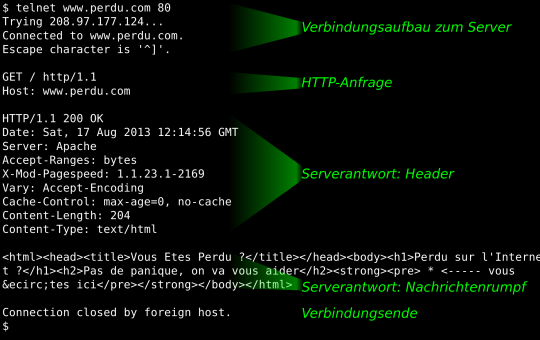
\includegraphics[width=0.6\textwidth]{img/http-anfrage.png}
  \caption{Beispiel einer HTTP-Transaktion}
\end{wrapfigure}

Bei jeder HTTP-Anfrage gibt es mehrere Abschnitte. Darunter den Abschnitt des
Verbindungsaufbaus zum Server
(\href{http://www.rvs.uni-bielefeld.de/~heiko/tcpip/tcpip_html_alt/kap_2_4.html}{TCP-Handshake}),
die HTTP-Anfrage, die Serverantwort geteilt in HTTP-Header und den HTTP-Body als
auch den Verbindungsabbau. Um \acrshort{acr:rest}-Endknoten anzusteuern sind
jedoch die beiden Serverantwortbereiche von Bedeutung. Der HTTP-Body enthält je
nach Anfragemethode einen Inhalt (Content). Im HTTP-Header dagegen stehen
Informationen über den Server bzw. dem Client, die Verschlüsselung zwischen den
beiden Kommunikationspartnern und einen HTTP-Statuscode der Auskunft über die
Aktion des Aufrufs wiedergibt.

Der Inhalt bzw. die Ressource im HTTP-Body kann beispielsweise eine PDF-Datei
oder ein Bild im .PNG-Format sein. Jedoch ist es auch möglich, einfachen Text zu
übermitteln der eine (semi-)Struktur aufweist. Infrage kommt bei solchen
Datenstrukturen beispielsweise \acrfull{acr:json} oder \acrfull{acr:xml}, wobei
sich \acrshort{acr:json} durch seine semi-Struktur überwiegend durchgesetzt hat.

Um welche Art bzw. Dateityp es sich bei einer Ressource handelt wird über den
Content-Type oder auch Media-Type im HTTP-Header definiert. Mögliche Werte für
den
\href{http://www.iana.org/assignments/media-types/media-types.xhtml}{Content-Type}
wird von der \acrfull{acr:iana} standardisiert und veröffentlicht.

Über das Kommandozeilenprogramm cURL ist es möglich alle Anfragemethoden mit
einem HTTP-Body zielgerichtet an einen Server zu senden. Nachfolgend werden
exemplarisch die Befehle je nach Anfragemethode dokumentiert. Dabei handelt es
sich um Temperaturdaten. Alle Befehle die über das Terminal (Bash) ausgeführt
werden richten sich an einen Flucky-Server in der Version 0.0.3.

% >------------------------------------------------------<
\subsubsection{GET}%
\label{sec:rest.ansteuern.get}

Als Vorgabe verwendet cURL automatisch die Anfragemethode GET. Wird in einem
Terminal der nachfolgende Befehl abgesetzt, ruft cURL die über das erste
Argument mitgegebene Adresse auf und gibt den HTTP-Body (Inhalt) in dem Terminal
aus.

\inputbash{./bash/curl-get.sh}

Der HTTP-Body enthält ein \acrshort{acr:json}. Wobei das \acrshort{acr:json} ein
Text ist und über jeden herkömmlichen Parser eingelesen werden kann. Über den
einfachen Aufruf von cURL werden keine zusätzlichen Informationen über die
Kommunikationspartner, die Verschlüsselung oder den HTTP-Statuscode ausgegeben.
Erweiterte Informationen über den Vorgang erhält man mit dem Flag \texttt{-v}
oder auch \texttt{--verbose}.

% >------------------------------------------------------<
\subsubsection{POST}%
\label{sec:rest.ansteuern.post}

cURL ist ebenfalls in der Lage Daten an einen Server zu übermitteln. Dazu werden
cURL zwei Parameter übergeben, einen zum setzten der Anfragemethode
\texttt{--request POST} und zu zweiten \texttt{--data} eine Datei oder ein
Inhalt (Content) der übermittelt werden soll.

Im nachfolgenden Beispiel werden zwei erfasste Datensätze, die als
\acrshort{acr:json} strukturiert sind, an einen Flucky-Server übermittelt. Dabei
ist darauf zu achten, dass der \acrshort{acr:rest}-Knoten die Anfragemethode
unterstützt (siehe Tabellenverzeichnis) und der HTTP-Body bzw. Inhalt oder auch
Content richtig strukturiert ist, sodass der Server die Daten einwandfrei parsen
kann.

\inputbash{./bash/curl-post.sh}

Dabei ist zu erkennen, dass die Objekt-Eigenschaft \texttt{temperature\_id} im
zweiten JSON-Objekt fehlt. Da JSON semistrukturiert ist, können
Objekt-Eigenschaften leer oder auch einfach weg gelassen werden. Der Server
versucht fehlende Informationen selber zu ermitteln oder sendet dem Client einen
400 HTTP-Statuscode] zurück.

HTTP-Statuscodes geben dem Client eine Rückmeldung über den Status ihrer
HTTP-Anfrage. Bei einem HTTP-Statuscode der nicht zu den 200er Klasse gehört
gibt cURL einen Fehler direkt im Terminal bzw. der Konsole aus.

% >------------------------------------------------------<
\subsubsection{PUT}%
\label{sec:rest.ansteuern.put}

Ähnlich wie bei der Anfragemethode POST werden auch bei der Methode PUT Daten
vom Client an den Server übermittelt. Allerdings richtet sich die Anfragemethode
PUT an das Aktualisieren einer Ressource. Um cURL mitzuteilen einen PUT-Aufruf
abzusetzen kann das Flag \texttt{--request PUT} gesetzt werden. Kennt der
Anwender die eindeitige UUID der Ressource lässt sich der REST-Endknoten oft
sematisch ableiten. Der Flucky-Server stellt ebenso einen REST-Endknoten zum
aktualisieren von Ressourcen bereit. Siehe dazu das Tabellenverzeichnis.

Im nachfolgendem Beispiel wird nur der Wert des Datensatzes mit der UUID
c7299f17-78da-43c6-be1c-5c99ac909807 von 34.50 auf 30.50 aktualisiert. Es
unterscheidet sich hier zum HTTP-Body der Anfragemethode POST, dass nicht alle
Objekt-Eigenschaften vorhanden sind, sondern nur die die aktualisiert werden
sollen.

\inputbash{./bash/curl-put.sh}

% >------------------------------------------------------<
\subsubsection{DELETE}%
\label{sec:rest.ansteuern.delete}

Um Ressourcen zu löschen unterstützt cURL ebenso die Anfragemethode DELETE,
\texttt{--request DELETE}. Dabei muss kein HTTP-Body angegeben werden, sondern
nur der REST-Endknoten an dem der Aufruf ausgeführt werden soll. Beim absenden
eines Aufrufs mit der Anfragemethode DELETE werden alle Daten gelöscht, die über
die Anfragemethode GET abgerufen werden können. Daher ist es mit Vorsicht zu
genießen einen DELETE-Aufruf abzusetzen! Im Tabellenverzeichnis sind alle
REST-Endknoten die die Anfragemethode DELETE unterstützten aufgelistet.

Nachfolgend wird der Temperatur-Datensatz mit der UUID
c7299f17-78da-43c6-be1c-5c99ac909807 gelöscht.

\inputbash{./bash/curl-delete.sh}

% #>----------------------------------------------------<#
\subsection{JSON}%
\label{sec:rest.json}

Wie bereits im Kapitel REST-Endknoten erwähnt wird \acrshort{acr:json} als
Datenstruktur verwendet. Nachfolgend werden alle Datenstrukturen in
\acrshort{acr:json}-Format abgebildet und beschrieben.

% >------------------------------------------------------<
\subsubsection{camera equals}%
\label{sec:rest.json.camera_equals}

Das nachfolgende \acrshort{acr:json}-Array enthält mehrere
\acrshort{acr:json}-Objekte. Jedes Objekt bildet einen Datensatz ab bestehend
aus mehreren Objekt-Eigenschaften. Der Datensatz beschreibt einen Vorgang bei
dem ein Objekt mittels Kamera erfasst wird und wie hoch die prozentuale
Übereinstimmung mit einem anderen Objekt ist.

\begin{jsoncode}
  [
    {
      "camera_equal_id":"d1103459-375b-46dc-8508-67eff7b56802",
      "similarity":"0.41",
      "camera_equal_date":"2018-12-30T12:24:28.132417Z",
      "sensor_id":"c2987fa3-288e-4765-bbc8-0927df149e83"
    },
    {
      "similarity":"0.34",
      "camera_equal_date":"2018-12-30T12:24:28.132417Z",
      "sensor_id":"c2987fa3-288e-4765-bbc8-0927df149e83"
    }
  ]
\end{jsoncode}

\begin{table}[H]
  \begin{tabularx}{\textwidth}{lX}
    \textbf{Objekt-Eigenschaft} & \textbf{Beschreibung}                                                                     \\ \toprule
    camera\_equal\_id           & Eindeutige UUID um die Ressource zu identifizieren. Bei der Anfragemethode POST optional  \\
    similarity                  & Prozentuale Trefferquote beim Vergleich von Objekten                                      \\
    camera\_equal\_date         & Datum an dem das Objekt erfasst wurde                                                     \\
    sensor\_id                  & Eindeutige UUID des Sensors, der das Objekt gescannt hat                                  \\
  \end{tabularx}
\end{table}

% >------------------------------------------------------<
\subsubsection{camera size}%
\label{sec:rest.json.camera_size}

Das nachfolgende JSON-Array enthält mehrere JSON-Objekte. Jedes Objekt bildet
einen Datensatz ab bestehend aus mehreren Objekt-Eigenschaften. Der Datensatz
beschreibt einen Vorgang bei dem ein Objekt mittels Kamera auf Größe erfasst
wird.

\begin{jsoncode}
  [
    {
      "camera_size_id":"f1ec28e3-8ce3-4224-bbc5-8f4005dd4f79",
      "width":"412",
      "height":"145",
      "camera_size_date":"2018-12-30T12:24:28.132417Z",
      "sensor_id":"c2987fa3-288e-4765-bbc8-0927df149e83"
    },
    {
      "width":"341",
      "height":"244",
      "camera_size_date":"2018-12-30T12:24:28.132417Z",
      "sensor_id":"c2987fa3-288e-4765-bbc8-0927df149e83"
    }
  ]
\end{jsoncode}

\begin{table}[H]
  \begin{tabularx}{\textwidth}{lX}
    \textbf{Objekt-Eigenschaft} & \textbf{Beschreibung}                                                                     \\ \toprule
    camera\_size\_id            & Eindeutige UUID um die Ressource zu identifizieren. Bei der Anfragemethode POST optional  \\
    width                       & Breite des Objekts                                                                        \\
    height                      & Höhe des Objekts                                                                          \\
    camera\_size\_date          & Datum an dem das Objekt erfasst wurde                                                     \\
    sensor\_id                  & Eindeutige UUID des Sensors, der das Objekt gescannt hat                                  \\
  \end{tabularx}
\end{table}

% >------------------------------------------------------<
\subsubsection{checkpoints}%
\label{sec:rest.json.checkpoints}

Das nachfolgende JSON-Array enthält mehrere JSON-Objekte. Jedes Objekt bildet
einen Datensatz ab bestehend aus mehreren Objekt-Eigenschaften. Der Datensatz
beschreibt einen Vorgang bei dem ein Objekt einen Schalter passiert hat. Dies
kann Beispielsweise zur Warenerkennug auf einem Fließband dienen.

\begin{jsoncode}
  [
    {
      "checkpoint_id":"fb22abb2-8575-41ec-9b33-485e75697e08",
      "checkpoint_date":"2018-10-20T11:24:28.132417Z",
      "rfid":"eeb7ee4f-3f4",
      "product_id":"4957aa35-827c-4c3d-a15f-de1f31f19723",
      "sensor_id":"c2987fa3-288e-4765-bbc8-0927df149e83"
    },
    {
      "checkpoint_id":"4d3c2b1f-a9dd-4f8d-ac3f-5006812234a3",
      "checkpoint_date":"2018-10-20T11:28:28.132417Z",
      "rfid":"fd0ea90c-7c2",
      "product_id":"917a44ca-2068-40fe-bef0-55b636047b9f",
      "sensor_id":"c2987fa3-288e-4765-bbc8-0927df149e83"
    }
  ]
\end{jsoncode}

\begin{table}[H]
  \begin{tabularx}{\textwidth}{lX}
    \textbf{Objekt-Eigenschaft} & \textbf{Beschreibung}                                                                     \\ \toprule
    checkpoint\_id              & Eindeutige UUID um die Ressource zu identifizieren. Bei der Anfragemethode POST optional  \\
    checkpoint\_date            & Datum an dem das Objekt den Schalter passiert hat                                         \\
    rfid                        & ID des RFID-Chips                                                                         \\
    product\_id                 & ID des Produktes, das den Schalter passiert hat                                           \\
    sensor\_id                  & Eindeutige UUID des Sensors, der das Objekt gescannt hat                                  \\
  \end{tabularx}
\end{table}

% >------------------------------------------------------<
\subsubsection{failnoises}%
\label{sec:rest.json.failnoises}

Das nachfolgende JSON-Array enthält mehrere JSON-Objekte. Jedes Objekt bildet
einen Datensatz ab bestehend aus mehreren Objekt-Eigenschaften. Der Datensatz
beschreibt einen Vorgang wie oft ein Sensor zwischen zwei Zeiträumen
Fehlgeräusche ermittelt hat.

\begin{jsoncode}
  [
    {
      "failnoise_id":"53ba3985-9e5e-4f2e-8171-96502d750436",
      "failnoise_counter":"32",
      "failnoise_start_date":"2018-10-20T11:24:28.132417Z",
      "failnoise_end_date":"2018-10-20T11:24:32.132417Z",
      "failnoise_date":"2018-12-30T11:24:32.132417Z",
      "sensor_id":"c2987fa3-288e-4765-bbc8-0927df149e83"
    },
    {
      "failnoise_counter":"72",
      "failnoise_start_date":"2018-10-18T14:12:12.132417Z",
      "failnoise_end_date":"2018-10-19T14:18:24.132417Z",
      "failnoise_date":"2018-12-30T11:24:32.132417Z",
      "sensor_id":"c2987fa3-288e-4765-bbc8-0927df149e83"
      }
  ]
\end{jsoncode}

\begin{table}[H]
  \begin{tabularx}{\textwidth}{lX}
    \textbf{Objekt-Eigenschaft} & \textbf{Beschreibung}                                                                     \\ \toprule
    failnoise\_id               & Eindeutige UUID um die Ressource zu identifizieren. Bei der Anfragemethode POST optional  \\
    failnoise\_counter          & Anzahl der ermittelten Fehlgeräusche                                                      \\
    failnoise\_start\_date      & Startdatum der Messung                                                                    \\
    failnoise\_end\_date        & Enddatum der Messung                                                                      \\
    failnoise\_date             & Datum an dem die Messung erfasst wurde                                                    \\
    sensor\_id                  & Eindeutige UUID des Sensors der die Messung durchgeführt hat                              \\
  \end{tabularx}
\end{table}

% >------------------------------------------------------<
\subsubsection{humidity}%
\label{sec:rest.json.humidity}
Das nachfolgende JSON-Array enthält mehrere JSON-Objekte. Jedes Objekt bildet einen Datensatz ab bestehend aus mehreren Objekt-Eigenschaften. Der Datensatz beschreibt eine Messung der Luftfeuchtigkeit.

\begin{jsoncode}
  [
    {
      "humidity_id":"d53bd365-5f9f-4b8a-a4be-74e7e8f209ac",
      "humidity_value":"0.55",
      "humidity_date":"2018-10-15T23:24:28.132417Z",
      "sensor_id":"c2987fa3-288e-4765-bbc8-0927df149e83"
    },
    {
      "humidity_value":"0.57",
      "humidity_date":"2018-10-15T23:32:28.132417Z",
      "sensor_id":"c2987fa3-288e-4765-bbc8-0927df149e83"
    }
  ]
\end{jsoncode}

\begin{table}[H]
  \begin{tabularx}{\textwidth}{lX}
    \textbf{Objekt-Eigenschaft} & \textbf{Beschreibung}                                                                     \\ \toprule
    humidity\_id                & Eindeutige UUID um die Ressource zu identifizieren. Bei der Anfragemethode POST optional  \\
    humidity\_value             & Luftfeuchtigkeit                                                                          \\
    humidity\_date              & Datum an dem die Luftfeuchtigkeit gemessen wurde                                          \\
    sensor\_id                  & Eindeutige UUID des Sensors der die Messung durchgeführt hat                              \\
  \end{tabularx}
\end{table}

% >------------------------------------------------------<
\subsubsection{knocks}%
\label{sec:rest.json.knocks}

Das nachfolgende JSON-Array enthält mehrere JSON-Objekte. Jedes Objekt bildet
einen Datensatz ab bestehend aus mehreren Objekt-Eigenschaften. Der Datensatz
beschreibt wie oft Geräusche innerhalb eines Messzeitraums erfasst wurden.

\begin{jsoncode}
  [
    {
      "knock_id":"d53bd365-5f9f-4b8a-a4be-74e7e8f209ac",
      "knock_counter":"32",
      "knock_start_date":"2018-10-15T23:24:28.132417Z",
      "knock_end_date":"2018-10-15T23:24:32.132417Z",
      "knock_date":"2018-12-30T23:32:28.132417Z",
      "sensor_id":"c2987fa3-288e-4765-bbc8-0927df149e83"
    },
    {
      "knock_counter":"38",
      "knock_start_date":"2018-10-15T23:32:12.132417Z",
      "knock_end_date":"2018-10-15T23:34:24.132417Z",
      "knock_date":"2018-12-30T23:32:28.132417Z",
      "sensor_id":"c2987fa3-288e-4765-bbc8-0927df149e83"
      }
  ]
\end{jsoncode}

\begin{table}[H]
  \begin{tabularx}{\textwidth}{lX}
    \textbf{Objekt-Eigenschaft} & \textbf{Beschreibung}                                                                     \\ \toprule
    humidity\_id                & Eindeutige UUID um die Ressource zu identifizieren. Bei der Anfragemethode POST optional  \\
    knock\_counter              & Anzahl der ermittelten Fehlgeräusche                                                      \\
    knock\_start\_date          & Datum an dem die Messung gestartet wurde                                                  \\
    knock\_end\_date            & Datum an dem die Messung beendet wurde                                                    \\
    knock\_date                 & Datum an dem die Messung erfasst wurde                                                    \\
    sensor\_id                  & Eindeutige UUID des Sensors der die Messung durchgeführt hat                              \\
  \end{tabularx}
\end{table}

% >------------------------------------------------------<
\subsubsection{particulates10 und particulates25}%
\label{sec:rest.json.particulates}

Das nachfolgende JSON-Array enthält mehrere JSON-Objekte. Jedes Objekt bildet
einen Datensatz ab bestehend aus mehreren Objekt-Eigenschaften. Dieses
JSON-Array kann für alle REST-Endpunkte von particulates10 und particulates25
benutzt werden. Der Datensatz beschreibt die Messung der
Feinstaubpartikelbelastung an einem Messzeitpunkt. Dabei wird hier in die Größen
der Feinstaubpartikel in 10µ und 25µ unterschieden.

\begin{jsoncode}
  [
    {
      "particulate_id":"94339e1f-1591-471c-970c-682b9e535b71",
      "particulate_value":"0.50",
      "particulate_date":"2018-12-29T20:31:28.132417Z",
      "sensor_id":"c2987fa3-288e-4765-bbc8-0927df149e83"
    },
    {
      "particulate_id":"15fe00f4-61bc-4860-8f90-072f0e2184d8",
      "particulate_value":"2.60",
      "particulate_date":"2018-12-29T20:32:28.132417Z",
      "sensor_id":"c2987fa3-288e-4765-bbc8-0927df149e83"
    }
  ]
\end{jsoncode}

\begin{table}[H]
  \begin{tabularx}{\textwidth}{lX}
    \textbf{Objekt-Eigenschaft} & \textbf{Beschreibung}                                                                     \\ \toprule
    particulate\_id             & Eindeutige UUID um die Ressource zu identifizieren. Bei der Anfragemethode POST optional  \\
    particulate\_value          & Feinstaubpartikelbelastung                                                                \\
    particulate\_date           & Datum an dem die Messung erfasst wurde                                                    \\
    sensor\_id                  & Eindeutige UUID des Sensors der die Messung durchgeführt hat                              \\
  \end{tabularx}
\end{table}

% >------------------------------------------------------<
\subsubsection{temperature}%
\label{sec:rest.json.temperature}

Das nachfolgende JSON-Array enthält mehrere JSON-Objekte. Jedes Objekt bildet
einen Datensatz ab bestehend aus mehreren Objekt-Eigenschaften. Ein Datensatz
beschreibt die Messung der Temperatur durch einen Sensor an einem Zeitpunkt.

\begin{jsoncode}
  [
    {
      "temperature_id":"c7299f17-78da-43c6-be1c-5c99ac909807",
      "temperature_value":"34.50",
      "temperature_date":"2018-10-15T20:31:28.132417Z",
      "sensor_id":"c2987fa3-288e-4765-bbc8-0927df149e83"
    },
    {
      "temperature_value":"34.00",
      "temperature_date":"2018-12-30T22:31:28.132417Z",
      "sensor_id":"c2987fa3-288e-4765-bbc8-0927df149e83"
    }
  ]
\end{jsoncode}

\begin{table}[H]
  \begin{tabularx}{\textwidth}{lX}
    \textbf{Objekt-Eigenschaft} & \textbf{Beschreibung}                                                                     \\ \toprule
    temperature\_id             & Eindeutige UUID um die Ressource zu identifizieren. Bei der Anfragemethode POST optional  \\
    temperature\_value          & Erfasste Temperatur                                                                       \\
    temperature\_date           & Datum an dem die Messung erfasst wurde                                                    \\
    sensor\_id                  & Eindeutige UUID des Sensors der die Messung durchgeführt hat                              \\
  \end{tabularx}
\end{table}

% >------------------------------------------------------<
\subsubsection{throughputs}%
\label{sec:rest.json.throughputs}

Das nachfolgende JSON-Array enthält mehrere JSON-Objekte. Jedes Objekt bildet
einen Datensatz ab bestehend aus mehreren Objekt-Eigenschaften. Ein Datensatz
beschreibt die Messung einer durchschnittlichen Durchflussmenge innerhalb eines
Messzeitraums.

\begin{jsoncode}
  [
    {
      "throughput_id":"a6926bb4-e2d8-428b-960a-d20a05df1f87",
      "throughput_average":"343.52",
      "throughput_start_date":"2018-11-16T20:31:28.132417Z",
      "throughput_end_date":"2018-11-16T20:35:28.132417Z",
      "throughput_date":"2018-12-30T20:42:28.132417Z",
      "sensor_id":"c2987fa3-288e-4765-bbc8-0927df149e83"
    },
    {
      "throughput_average":"310.52",
      "throughput_start_date":"2018-11-16T20:38:28.132417Z",
      "throughput_end_date":"2018-11-16T20:42:28.132417Z",
      "throughput_date":"2018-12-30T20:42:28.132417Z",
      "sensor_id":"c2987fa3-288e-4765-bbc8-0927df149e83"
    }
  ]
\end{jsoncode}

\begin{table}[H]
  \begin{tabularx}{\textwidth}{lX}
    \textbf{Objekt-Eigenschaft} & \textbf{Beschreibung}                                                                     \\ \toprule
    throughput\_id              & Eindeutige UUID um die Ressource zu identifizieren. Bei der Anfragemethode POST optional  \\
    throughput\_average         & Erfasste Temperatur                                                                       \\
    throughput\_start\_date     & Datum an dem die Messung gestartet wurde                                                  \\
    throughput\_stop\_date      & Datum an dem die Messung beendet wurde                                                    \\
    temperature\_date           & Datum an dem die Messung erfasst wurde                                                    \\
    sensor\_id                  & Eindeutige UUID des Sensors der die Messung durchgeführt hat                              \\
  \end{tabularx}
\end{table}


\section{Installation von Docker}%
\label{sec:docker}

Der Flucky-Server besitzt den Vorteil, dass durch die Programmiersprache Golang
nur \textbf{eine} Binary, ohne zusätzlich abhängige Bibliotheken, durch den
Kompiler kompiliert wird. Dieser ausführbare Datei ist somit sehr einfach auf
anderen Systemen auszuführen da keine zusätzlichen Bibliotheken gebraucht
werden. Momentan wird die Binary jedoch ausschließlich für x86\_64 Linux
Architekturen kompiliert. Es gibt zusätzlich neben der Binary ein Docker-Image.
Dadurch dieses Image ist es möglich die Binary auf anderen Architektur laufen zu
lassen.

Ein Docker-Image ermöglich das einfache ausrollen einer Applikation in eine
bestehende Umgebung. Applikationen die auf Docker-Images basieren lassen sich in
einer Cloud-Architektur ohne große Hürden skalieren. Allerdings muss die
Applikation die Vorraussetzung erfüllen, nicht mit zustandsbehafteten Daten zu
arbeiten. Zustandsbehaftete Daten sind jene, die über eine Session oder eine
Transaktion übermittelt werden. Dies ist der Fall bei Datenbanken -
\href{https://de.wikipedia.org/wiki/ACID}{ACID}. Der Flucky-Server jedoch ist
genau auf den Umstand vorbreitet mit zustandslose Daten zu arbeiten. Flucky
lässt sich daher horizontal als auch vertikal skalieren.

% #>----------------------------------------------------<#
\subsection{Vorraussetzung}%
\label{sec:docker.vorraussetzung}

Als Vorraussetzung wird das Kernelmodul cgroups \footcite{cgroups} benötigt.
Daher werden gleich alle Betriebssysteme die nicht auf einem Linux Kernel in der
Version 2.26+ basieren für die Installation von Docker ausgeschlossen. Es gibt
jedoch auch für nicht Linux Kernel basierende Betriebssysteme wie Windows, Apple
oder BSD die Möglichkeit Docker zu verwenden. Dazu muss eine Virtuelle-Maschine
basierend auf dem Linux Kernel installiert werden.\footcite{moby}

% #>----------------------------------------------------<#
\subsection{Installationsschritte}%
\label{sec:docker.installation}

Um Docker nun, je nach Diverat, zu installieren gibt es mehrere Möglichkeiten.
Die einfachste Möglichkeit ist es Docker aus einem Entwickler-Repository zu
installieren, jedoch steht dieses nicht für jedes Diverat zur Verfügung.
Alternativ dazu kann das offizielle Repository des Diverats genutzt werden.

% >------------------------------------------------------<
\subsubsection{Arch Linux}%
\label{sec:docker.installation.arch-linux}

Unter Arch Linux kann Docker aus den offiziellen Paketquellen bezogen werden.
Bei Arch Linux handelt es sich um ein \Gls{gls:rolling-release} System. Dadurch
können schnell Aktualisierungen von Docker auf dem System eingespielt werden.

\inputbash{./bash/docker-arch-linux.sh}

% >------------------------------------------------------<
\subsubsection{Debian/Ubuntu/Linux Mint}%
\label{sec:docker.installation.debian}

Bei Debian Diveraten ist in den Paketquellen eine sehr alte Version von Docker
hinterlegt. Aus dem Grund muss ein PPA ("Personal Package Archive") hinterlegt
werden um von dort Docker als Softwarepaket im .deb Format zu beziehen und zu
installieren

\inputbash{./bash/docker-debian.sh}

% >------------------------------------------------------<
\subsubsection{Fedora/CentOS/RHEL}%
\label{sec:docker.installation.fedora}

Bei Fedora Diveraten ist es ähnlich wie bei Debian Diveraten. Hier muss auch ein
zusätzliches Packages Archive für Docker hinzugefügt werden um die aktuellsten
Versionen von Docker beziehen zu können.

\inputbash{./bash/docker-fedora.sh}


\section{Befehle von Docker im Überblick}%
\label{sec:docker-befehle}
Nachfolgend werden einige Befehle von Docker erklärt die essentiell für den täglichen Gebrauch sind.

% #>----------------------------------------------------<#
\subsection{docker run}%
\label{sec:docker-befehle.run}

Der \texttt{docker run} Befehl ist für Neulinge der mit Abstand schwierigste
Befehl für den Einstieg, dennoch komm niemand um ihn herum. Im Nachfolgenden
Beispiel wird ein nginx Server in der Version 1.13.8 basierend auf das
Dateisystem Alpine-Linux mittels Docker-Image erstellt und gestartet. Man
spricht ab diesem Zeitpunkt von einem Docker-Container. Für den Docker-Container
wird eine Weiterleitung der Ports 80 und 443 durch das Hostsystem eingerichtet.

\begin{bashcode}
  root@asterix:~# docker run --detach \
    --publish 80:80 \
    --publish 443:443 \
    nginx:1.13.8-alpine
\end{bashcode}

% #>----------------------------------------------------<#
\subsection{docker ps}%
\label{sec:docker-befehle.ps}

Der Befehl \texttt{docker ps} gibt eine Liste von allen Docker-Containern in der
Konsole aus. Dabei enthält die Liste die Container-ID, den Namen des
Docker-Images mit Version, der Befehl der in dem Container ausgeführt wird, wann
er erstellt und gestartet wurde und die Ports die vom Hostsystem an den
Container weitergeleitet wurden.

% #>----------------------------------------------------<#
\subsection{docker logs}%
\label{sec:docker-befehle.logs}

Mittels \texttt{docker logs} ist es möglich sich die Logeinträge eines
Docker-Containers in der Konsole ausgeben zu lassen. Das Flag \texttt{-f} oder
\texttt{--follow} ermöglich einen Stream zu öffnen um neue Logeinträge
fortlaufend in der Konsole zu erhalten. Mittels \texttt{Strg + C} kann der
Stream unterbrochen werden.

% #>----------------------------------------------------<#
\subsection{docker start/stop}%
\label{sec:docker-befehle.start-stop}

Möchte man einen Docker-Container stoppen kann dies mittels \texttt{docker stop}
realisiert werden. Dies ist nur möglich bei laufenden Containern.

\begin{bashcode}
   root@asterix:~# docker stop nginx
\end{bashcode}

Zum starten eines bereits erstellen Containers der gestoppt ist muss der Befehl
docker start verwendet werden.

\begin{bashcode}
  root@asterix:~# docker start nginx
\end{bashcode}

% #>----------------------------------------------------<#
\subsection{docker rm}%
\label{sec:docker-befehle.rm}

Um einen Container endgültig zu löschen wird docker rm verwendet. Hierbei ist es
allerdings notwendig, dass der Container zuvor gestoppt wurde. Über die Option
\texttt{-f} bzw. \texttt{--force} wird das ordentliche Herunterfahren des
Containers unterdrückt.

\begin{bashcode}
  root@asterix:~# docker rm nginx
\end{bashcode}

% #>----------------------------------------------------<#
\subsection{permission denied}%
\label{sec:docker-befehle.permission_denied}

Kommt es bei der Verwendung von Docker-Befehlen zu einem Fehler der auf
mangelnde Berechtigungen hinweist, dann muss der aktuelle Benutzer der Gruppe
docker hinzugefügt werden. Anschließend muss die Benutzer-Session durch erneutes
anmelden geladen werden.

\inputbash{./bash/docker-permission.sh}


\section{docker-compose}%
\label{sec:docker-compose}

Das CLI-Programm docker-compose ist ein Programm um mehrere Docker-Container zu
definieren, zu starten und zu verwalten. Das Programm nutzt
YAML-Dateien\footcite{yaml} zur Konfiguration der Container. Das Starten der
Container ist so über einen einzelnen Befehl möglich.

Nachfolgend wird eine Konfigurationsdatei \texttt{docker-compose.yml} erläutert
und der Umgang mit docker-compose beschrieben.

\begin{landscape}
  \inputbash{./bash/docker-compose.yaml}
\end{landscape}

Sicherlicht fragt man sich nun, was die geschweiften Klammern mit dem
Dollar-Zeichen bedeuten. Dies sind Bash-Umgebungsvariablen die in der
beiliegenden Datei \texttt{.env} definiert sind. Dies gibt bei größeren
\texttt{docker-compose.yml}-Files etwas Felxibilität zurück.

Die beiliegende \texttt{.env} Datei enhält folgenden Inhalt.

\begin{bashcode}
  SERVER_PORT=80
  DATABASE_DRIVER=postgres
  DATABASE_NAME=postgres
  DATABASE_SCHEMA=flucky
  DATABASE_USER=flucky
  DATABASE_PASSWORD=MyS3cretP4ssw0rd!
  PG_HOST=flucky-dev-db
  PG_INTERN_PORT=5432
  PG_EXTERN_PORT=5433
  PG_NAME=postgres
  PG_USER=postgres
  PG_PASSWORD=MyS3cretP4ssw0rd!
  TZ=Europe/Berlin
\end{bashcode}

% #>----------------------------------------------------<#
\subsection{Befehle von docker-compose im Überblick}%
\label{sec:docker-compose.befehle}

Da nun in einem beliebigen Verzeichnis die Dateien \texttt{.env} und
\texttt{docker-compose.yml} vorhanden sind kann das Programm
\texttt{docker-compose} zum Verwalten verwendet werden.

\begin{itemize}[itemsep=0pt]
  \item Die Container wie sie in dem YAML-File definiert sind zu starten reicht der Befehl \texttt{docker-compose up -d} aus. Das \texttt{-d} oder auch \texttt{--detached} steht dafür, dass der Container im Hintergrund gestartet werden soll.
  \item Über \texttt{docker-compose ps} erhält man eine ähnliche Ausgabe wie bei \texttt{docker ps}.
  \item Die Logfiles können mittels \texttt{docker-compose logs} im Terminal ausgegeben werden. Optional, wie auch bei \texttt{docker logs} kann das Flag \texttt{-f} oder auch \texttt{--follow} gesetzt werden um fortlaufend alle Logeinträge zu erhalten.
  \item Mittels \texttt{docker-compose stop} werden alle Container gestoppt. Optional kann hinter dem Befehl eine Liste von definierten Containern angegeben werden die gestoppt werden sollen. Zum Beispiel \texttt{docker-compose stop flucky-dev}. Gleiches gilt um Container zu löschen mittels \texttt{docker-compose rm}. Allerdings werden virtuelle Netzwerke oder Dateisysteme im YAML-File nicht per \texttt{docker-compose rm} gelöscht.
  \item Mit dem Befehl \texttt{docker-compose down} werden alle Container gestoppt, gelöscht und deren definierte Netzwerke und Dateisysteme entfernt. Der Befehl sollte jedoch mit Vorsicht zu genießen sein, denn wichtige Dateien die in virtuellen Dateisystemen gespeichert werden gehen dadurch verloren! Dies wäre laut der \texttt{docker-compose.yml} Datei alle Datenbank-Dateien.
\end{itemize}

% #>----------------------------------------------------<#
\subsection{Skalierung}%
\label{sec:docker-compose.skalierung}

Wie bereits erwähnt ist es möglich Container zu skalieren. Jedoch müssen diese
Zustandslos\footnotesize{zustandslosigkeit} sein. Der Flucky-Server ist darauf
ausgelegt und daher ist es möglich diesen zu skalieren. Da eine
\texttt{docker-compose.yml} als auch \texttt{.env}-Datei vorhanden ist, kann
\texttt{docker-compose} verwendet werden um den Flucky-Server zu skalieren.

Dazu reicht der Befehl \texttt{docker-compose scale flucky-deb-web=3} aus um
drei weitere Container zu starten.

\begin{bashcode}
  root@asterix:~/workspace/docker-dev-flucky# docker-compose scale flucky-dev-web=3
  Starting docker-dev-flucky_flucky-dev-web_1 ... done
  Creating docker-dev-flucky_flucky-dev-web_2 ... done
  Creating docker-dev-flucky_flucky-dev-web_3 ... done
\end{bashcode}
